
It is the UI that the user interacts with. The interface itself, as shown in \autoref{fig:figure1}, 
provides the user with a selection of input widgets in which, for the application of choosing, 
the user provides the information needed by the application for that part of the workflow. 
As seen in \autoref{fig:figure1}, on the left-hand side of the UI the user is presented with a selection of different applications used in the workflow. 
The input panel selection area consists of a number of choices:

\begin{enumerate}
  \item BIM: structure information, description and model generation.
  \item EVT: earthquake motions specification
  \item FEM: finite element application
  \item UQ: Uncertainty quantification: specification of the random variable parameters and UQ analysis options
  \item RES: results output.
\end{enumerate}


Selecting any of these will change the input panel. It is here that the user selects the actual application to be used and provides input for that application. 


\begin{figure}[!htbp]
  \centering {
    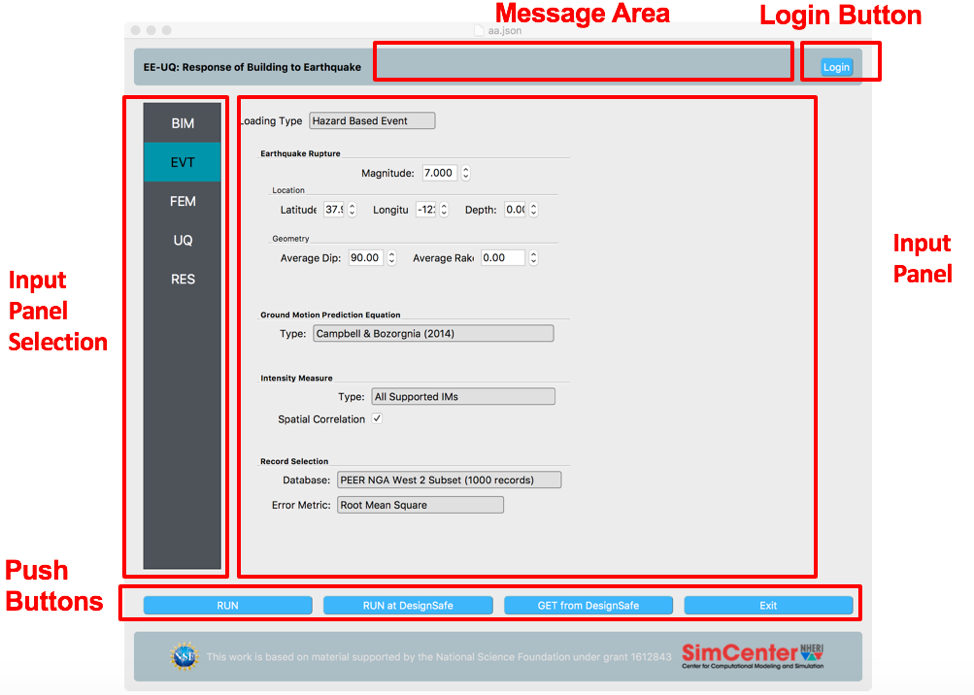
\includegraphics[width=0.8\textwidth]
    {figs/Figure1.png} }
  \caption{UI}
  \label{fig:figure1}
\end{figure}

Also in the UI is an area where status and error messages will be reported to you, a button to press to login (login is required only 
if you want to run the job at DesignSafe) and an area with a number of push buttons:
\begin{enumerate}
\item	RUN – to run the simulation of the user’s desktop machine.
\item	RUN at DesignSafe – to process the information, and send to DesignSafe where the job will be run on a supercomputer and results stored in your DesignSafe jobs folder.
\item	GET from DesignSafe – to obtain from DesignSafe your list of jobs and select from that list a job to download.
\item	Exit: to exit the application.
\end{enumerate}

The Screens presented to user when the first 3 of these buttons will be discussed in 2.5.

\section{BIM}
The user in the BIM panels defines the building. There are tabbed panels for this:
\begin{enumerate}
\item	GIM: general Information about the building. The panel presents 3 separate frames. A frame in which the user as shown in \autoref{fig:figure2}, 
defines information about the building. This includes the building type, name, year of construction, overall height, plan area, geographic location (needed for certain event types), etc. 
This information should be provided, as certain applications in the workflow that exist or are planned will need this information. 


In the other frames the user provides the building location and in the last panel the units. this may be needed in applications further down the workflow to ensure units are consistent throughout the applications. 

\begin{figure}[!htbp]
  \centering {
    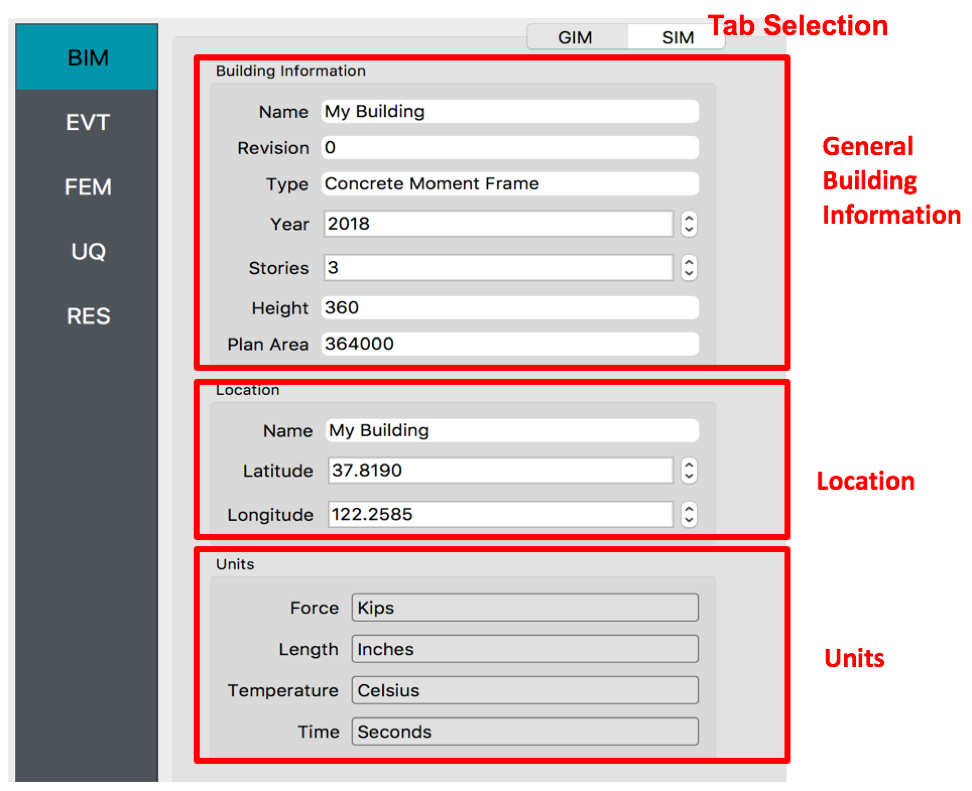
\includegraphics[width=0.8\textwidth]
    {figs/Figure2.png} }
  \caption{BIM}
  \label{fig:figure2}
\end{figure}


\item SIM: This panel is where the user defines the building. 
There is a drop-down menu that the user will use to select from a number of different modeling options. 
At present there is a single option, OpenSees. 
The panel that presents is as shown in \autoref{fig:figure3}. 
The user specifies the main script that contains the building model, 
a list of nodes that define a column line of interest for which the responses will be determined and an entry for the dimension of the model. 
Note the column nodes should be in order from ground floor through to roof (as drifts are calculated based on this). 
The spatial dimension is used to align the ground motion components in the EVENT file.

\begin{figure}[!htbp]
  \centering {
    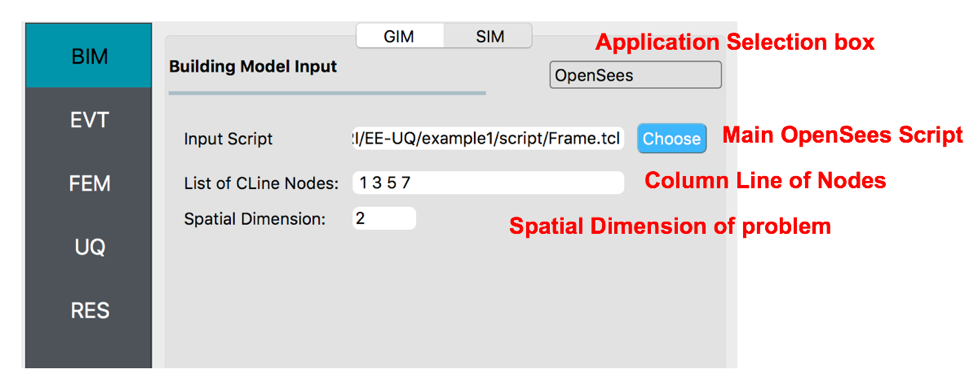
\includegraphics[width=0.8\textwidth]
    {figs/Figure3.png} }
  \caption{GIM}
  \label{fig:figure3}
\end{figure}

In the worked for version 1.1+ include code to describe the building in most general terms and allow 
the user to select from expert or machine learning systems that produce the building model file.

\end{enumerate}


\section{EVT (Event)}
The event panel presents the user with a drop-down menu with a list of available applications. 
Event applications are applications that given the building, 
and user supplied data to the specific applications input panel will generate a list of events for the building. 
There are a number of options:

\subsection{Multiple Event}

This is provided for the user to specify multiple existing SimCenter Event files. 
If more than one event is provided it is done to provide the UQ engine with a discrete set of events to choose from. 
It is not done with the intention of specifying that one event follows another. 
The panel presented initially to the user is as shown in \autoref{fig:figure4}.

\begin{figure}[!htbp]
  \centering {
    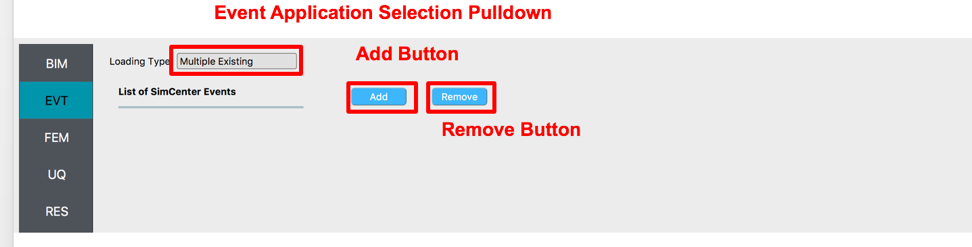
\includegraphics[width=0.8\textwidth]
    {figs/Figure4.png} }
  \caption{EVT}
  \label{fig:figure4}
\end{figure}

To add a new event, the user presses the Add button. 
This adds an event to the panel. 
Pressing the button multiple times will keep adding events to the panel. 
\autoref{fig:figure5} shows the state after the button has been pressed twice, 
and data entered for the ElCentro and Rinaldi Events.

\begin{figure}[!htbp]
  \centering {
    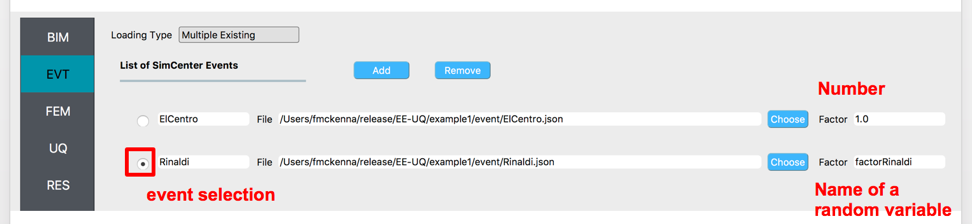
\includegraphics[width=0.8\textwidth]
    {figs/Figure5.png} }
  \caption{Adding new event}
  \label{fig:figure5}
\end{figure}


The user can enter the full path manually to the file or use the choose button, 
which brings up your typical file search screen. 
By default, a scaling factor of 1.0 is assigned to the event. 
The user can change this to another real value (AT PRESENT DO NOT USE INTEGER) or the user 
has the option of defining this to be a random variable by entering a name as shown for the second event. 
Note that this variable name must not start with a number, or contain any spaces or special characters, i.e. -, +,..

The Remove button is pressed to remove events. 
Once pressed it removes all button whose event selection box is highlighted.

\subsection{Multiple PEER Event}
This is provided for the user to specify multiple existing PEER 
(\href{http://peer.berkeley.edu}{http://peer.berkeley.edu}) ground motion files. 
For PEER events the user is required to specify the individual components for the EVENTS. 
The Add/Remove buttons at the top are to create and remove an event, as per 2.2.1. 
For the PEER events the user specifies components acting in the individual degree-of-freedom directions. 
The + and – add and remove components with the remove removing all components selected. 
Each component in a PEER event can have their own d=scale factor, again a number or a random variable.
\begin{figure}[!htbp]
  \centering {
    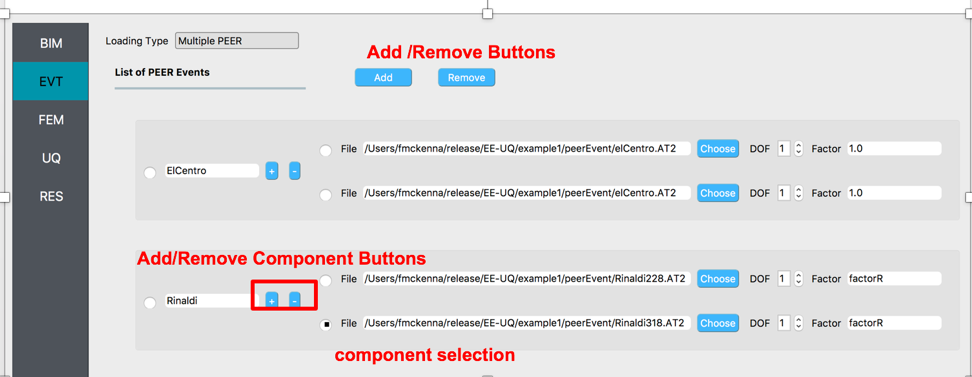
\includegraphics[width=0.8\textwidth]
    {figs/Figure6.png} }
  \caption{PEER event}
  \label{fig:figure6}
\end{figure}

\subsection{Hazard Based Event}
The panel for this event application is as shown in \autoref{fig:figure7}. 
This application implements a scenario-based (deterministic) seismic event. 
In this panel the user specifies an earthquake rupture (location, geometry and magnitude), a ground motion prediction equation, 
a record selection database and the intensity measure used for record selection. 
In the backend, this application relies on three other applications to perform seismic hazard analysis, 
intensity measures simulation (to create a simulated target spectrum), and ground motion record selection/scaling. 
Users interested in learning about those applications are referred to the documentation of 
the (\href{https://github.com/NHERI-SimCenter/GroundMotionUtilities/blob/master/Readme.md}{SimCenter ground motion utilities}).
\begin{figure}[!htbp]
  \centering {
    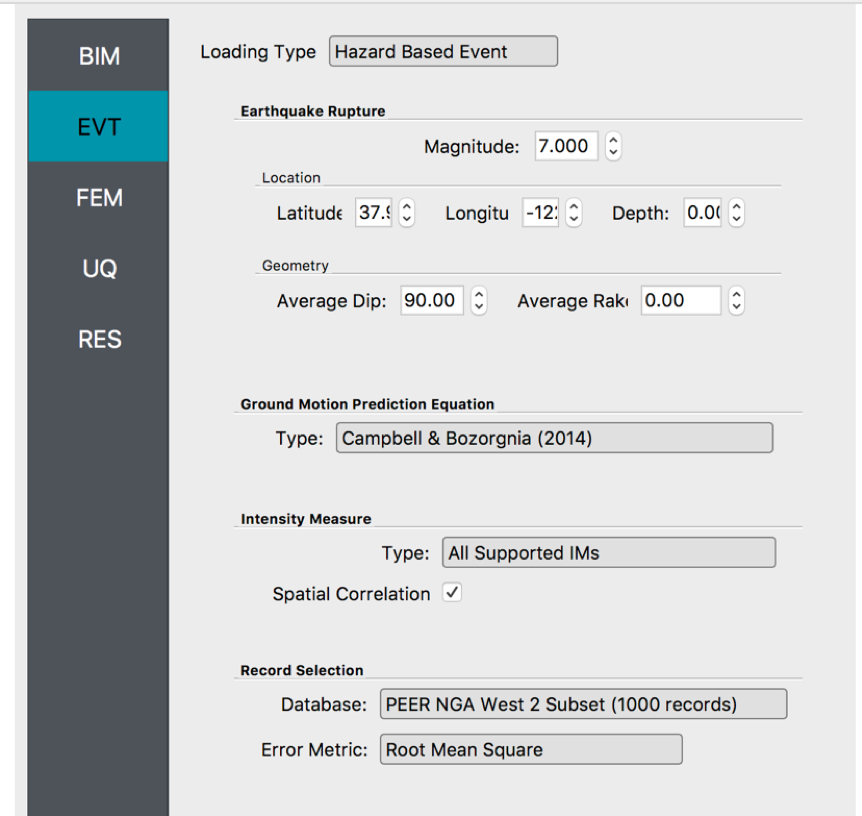
\includegraphics[width=0.8\textwidth]
    {figs/Figure7.png} }
  \caption{Hazard based event}
  \label{fig:figure7}
\end{figure}

\textcolor{red}{s3hark shows up here}



\subsection{User Application}
The final selection option is a user specific application. 
The user specifies the application name and the input file containing the specific input information 
needed by the application when it is running in the backend. 
As will be discussed, the user is also required when they use an additional application not provided, 
to edit the tools registry file. Here they must include a new event application with this same name 
and the location where that application can be found relative to the tools application directory. 
If running on DesignSafe, that application must of course be built and available on the Stampeded2 supercomputer. 
NOTE that given how DesignSafe runs the applications through Agave, this applications file permissions must be 
world readable and executable (as when user running their application through DesignSafe and Agave, they are not running as themselves!)

\begin{figure}[!htbp]
  \centering {
    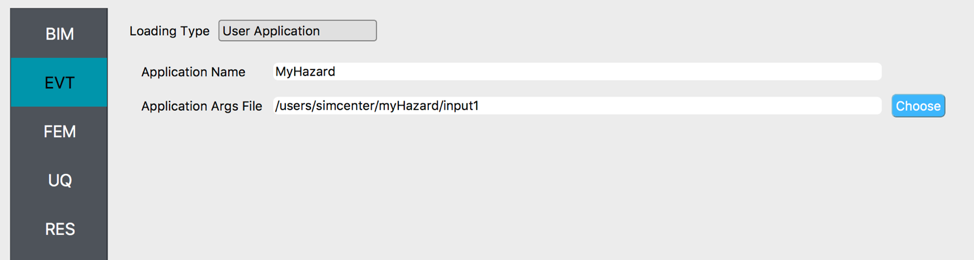
\includegraphics[width=0.8\textwidth]
    {figs/Figure8.png} }
  \caption{User defined event}
  \label{fig:figure8}
\end{figure}


\section{FEM}
The FEM panel is intended to present users with a selection of FEM applications that will take a building model 
generated by the BIM application and the EVENT from the event application and perform a deterministic simulation. 
At present there is only one application available, OpenSees and there is no application selection box. 
That will be modified in Version 1.1.0 to allow user to provide their own simulation application. 
This is not the standard OpenSees executable, but consists of a pre- and post-processor to take the 
BIM and EVENT file and use OpenSees to determine the response, returning these responses in an EDP. 
Presently the default EDPs are the relative floor displacements, total accelerations (ground motion + relative response) 
and inter-story drifts for column lines specified in the BIM panel.

\begin{figure}[!htbp]
  \centering {
    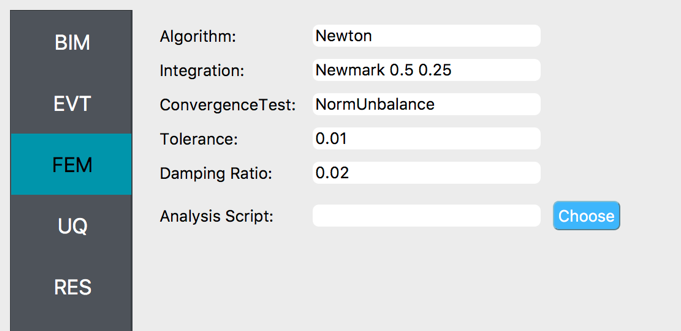
\includegraphics[width=0.8\textwidth]
    {figs/Figure9.png} }
  \caption{FEM}
  \label{fig:figure9}
\end{figure}

In the OpenSees FEM panel, the user specifies the algorithm, integration strategy, convergence test, tolerance and damping ratio. 
A default transient analysis script is run with these inputs. It is built for Version 3.0.0+ of OpenSees and uses a divide and conquer 
algorithm in event of a convergence failure issue. This new algorithm does not always work. The user is also able to specify their 
own analysis script to run instead of the default. When chosen the variables numStep and dt that are obtained from the EVENT 
should be assumed to have been set by the application before the script is run and can be used in your user defined script.

\section{UQ}
Throughout the input specification the user is defining variables. Many of these variables can be specified by the user to be 
random variables with a distribution on their values. It is in the UQ panel that the user specifies what these distributions are. 
It is also here that the user specifies what UQ engine, what UQ method and other inputs are for the UQ method. 
The panel is split into 2 tabs: Sampling Methods and Random Variables as shown in \autoref{fig:figure10}.

\begin{figure}[!htbp]
  \centering {
    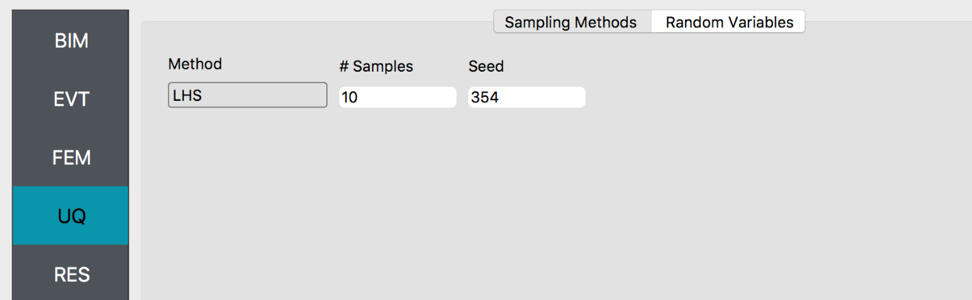
\includegraphics[width=0.8\textwidth]
    {figs/Figure10.png} }
  \caption{UQ}
  \label{fig:figure10}
\end{figure}


\subsection{Sampling Methods}
In the sampling methods the user selects the sampling method to use from the method dropdown. Currently this is limited to two options: 
Monte Carlo and Latin Hypercube Sampling (LHS). For the one selected, the user specifies the number of simulations to perform and the seed.

\subsection{Random Variables}
The Random Variable panel is where the user enters the random variables. Each random variable has a name associated with it, a distribution, 
and depending on the distribution a number of additional variables to specify. As with the other panels discussed, random variables can be 
added and removed using the added remove buttons. It should also be noted that the random variables should be created automatically 
when they are entered in previous screens. 


Some Notes:
\begin{itemize}
\item A current limitation of the tool is that it does not check for multiple random variables with the same name, nor does it remove a 
random variable if the random variable is removed, e.g. factor in an earthquake event is set to a number or a different OpenSees file is loaded. 
The user in such circumstances is required to manually remove the variable from the UQ
\item Also, do note that when initially created Random variables are assigned a constant type. 
The UQ engine will ignore any variables with such a type as they are not random.
\item When using OpenSees input files, this application will read any variable set with the pset command as a random variable and create a 
random variable for it when the user chooses the main file. See the example in example/script/Frame.tcl directory.
\end{itemize}


\begin{figure}[!htbp]
  \centering {
    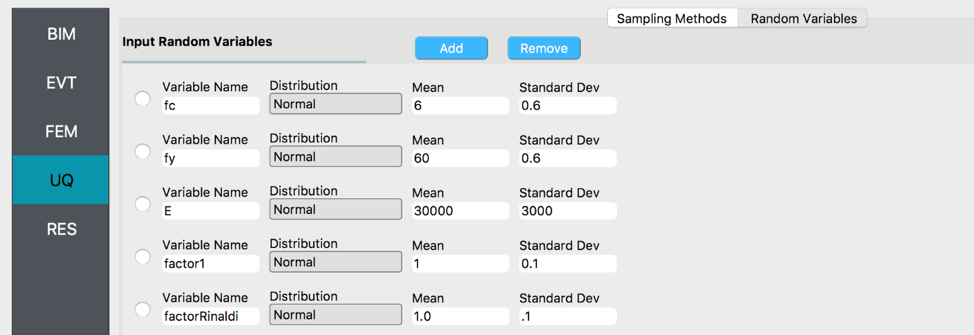
\includegraphics[width=0.8\textwidth]
    {figs/Figure11.png} }
  \caption{Random variables}
  \label{fig:figure11}
\end{figure}



\section{RES}

When the user hits the Run button, and assuming the results are successful. The results are presented here. 
A successful run or download of a job that ran successfully will result in 3 tabbed widgets being displayed in this panel. 
The first panel shows summary statistics: mean and stdDev values or min-max values if discrete set, i.e. multiple events
\begin{figure}[!htbp]
  \centering {
    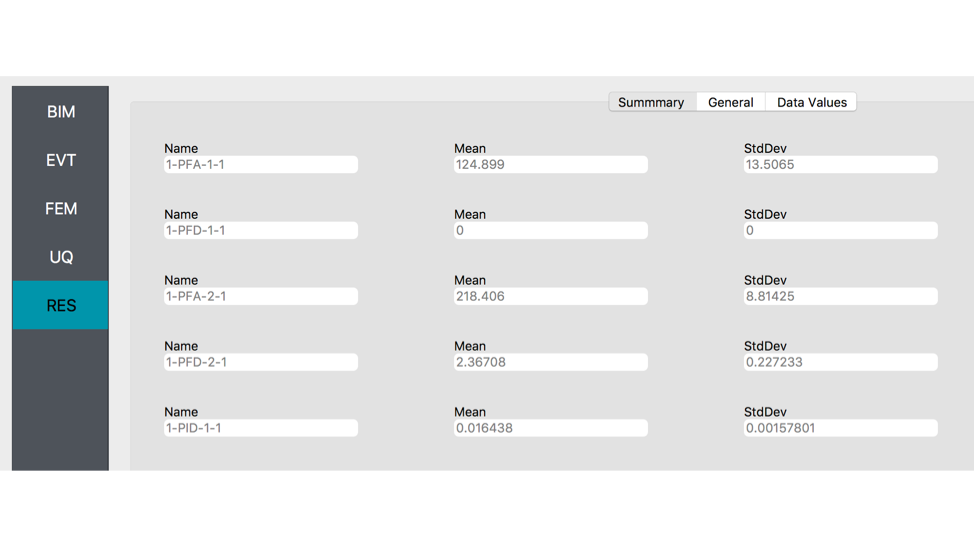
\includegraphics[width=0.8\textwidth]
    {figs/Figure12.png} }
  \caption{RES}
  \label{fig:figure12}
\end{figure}

The second panel shows the summary information.
\begin{figure}[!htbp]
  \centering {
    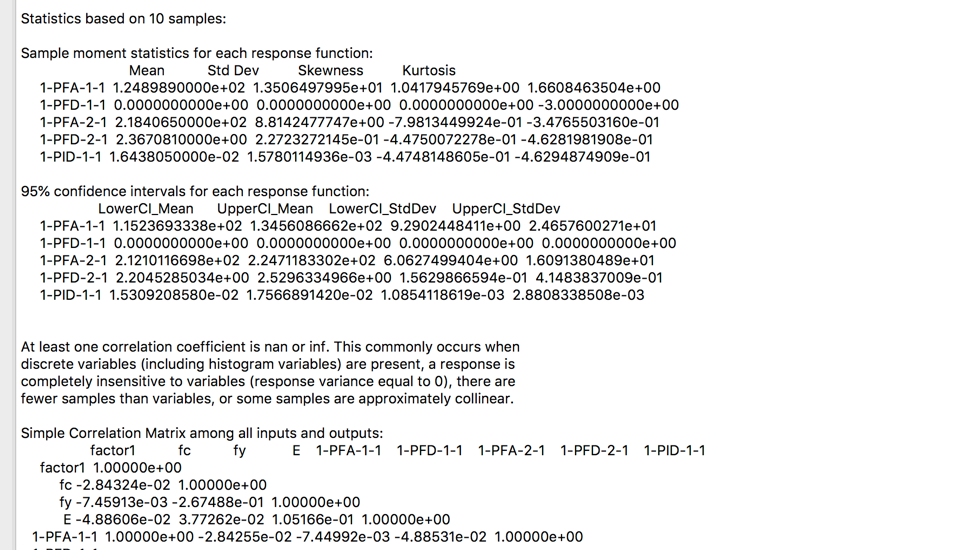
\includegraphics[width=0.8\textwidth]
    {figs/Figure13.png} }
  \caption{RES General tab}
  \label{fig:figure13}
\end{figure}

The third panel presents graphically and in tabular form the results. By selecting different columns with left and right mouse buttons in the table below the graphic, 
the information in the graph is changed. Selecting the left mouse button changes the Y axis, the right mouse changes the X axis. If the same column is selected 
using both left and right keys, the CDF and PDF is displayed. If last mouse press was with the left button, the PDF and if right the CDF.

As for the columns. You will see a column for each random variable the workflow came across. There may be more than you specified if the applications want the 
UQ engine to consider their own variables in the computation. The outputs at present are limited to:

\begin{itemize}
\item PFD peak relative floor displacement $1-PFD-FLOOR_CLINE$
\item PFA peak floor acceleration (relative + ground motion): $1-PFA-FLOOR-CLINE$
\item PID peak inter-story drift: $1-PID-STORY-CLINE$
\end{itemize}

\begin{figure}[!htbp]
  \centering {
    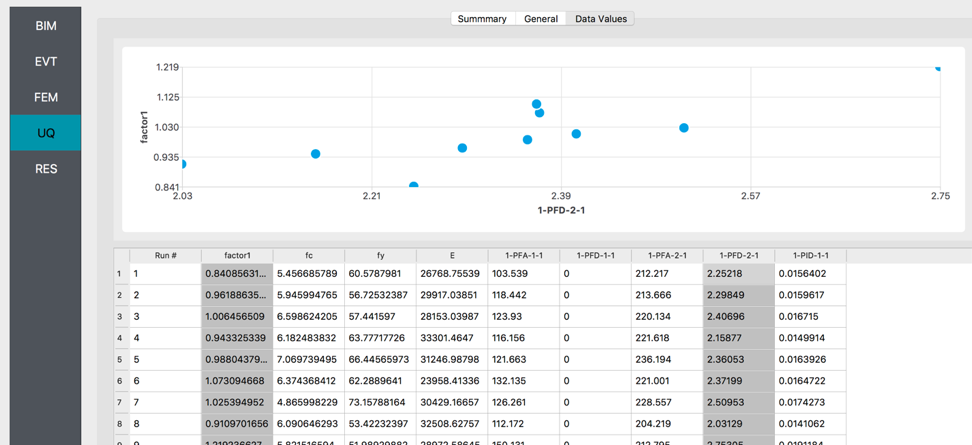
\includegraphics[width=0.8\textwidth]
    {figs/Figure14.png} }
  \caption{UQ Data Values}
  \label{fig:figure14}
\end{figure}



\section{Push Buttons}
There are a number of buttons in the Push Button area of \autoref{fig:figure1}:
\subsection{RUN – to run the simulation of the user’s desktop machine.}
\begin{figure}[!htbp]
  \centering {
    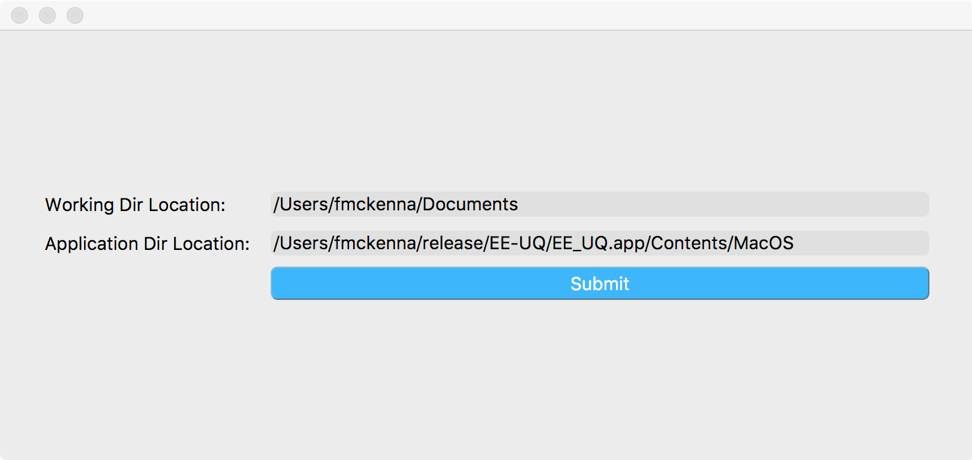
\includegraphics[width=0.8\textwidth]
    {figs/Figure15.png} }
  \caption{Run button}
  \label{fig:figure15}
\end{figure}
The window that pops up is as shown in \autoref{fig:figure15}. There are 2 entries and a push button: 

\begin{itemize}
\item Working Dir Location: specifies where the $EE_UQ$ application can create a “temporary” directory called tmp. SimCenter that the application 
creates when the submit button is pressed. The application creates this directory, copies files to it that the application needs as a result of your 
input (e.g. if you are using OpenSees input script, it will to the tmp. SimCenter directory copy that script, ALL FILES IN THAT DIRECTORY AND ALL FILES IN 
SUBDIRECTORIES OF THAT DIRECTORY GET COPIED SO DON’T PLACE THE SCRIPT IN HOME, DOWNLOADS, DOCUMENTS, ….
\item Application Dir Location: SHOULD NOT BE TOUCHED unless you are introducing your own applications or want to build and modify the 
applications provided with the tool. It is this directory the application tool looks to find the applications to run.
\end{itemize}


Finally, when inputs are finished the user hits submit button to start the backend job. If it runs the window will close and the RES 
panel will pop up on successful run. Do not press the submit button multiple times while waiting for it to close. We cannot guarantee 
what will happen and we did not disable the button in this release.

\subsection{RUN at DesignSafe}
Click this button to process the information, and send to DesignSafe where the job will be run on a supercomputer and results stored in your DesignSafe jobs folder.

\begin{figure}[!htbp]
  \centering {
    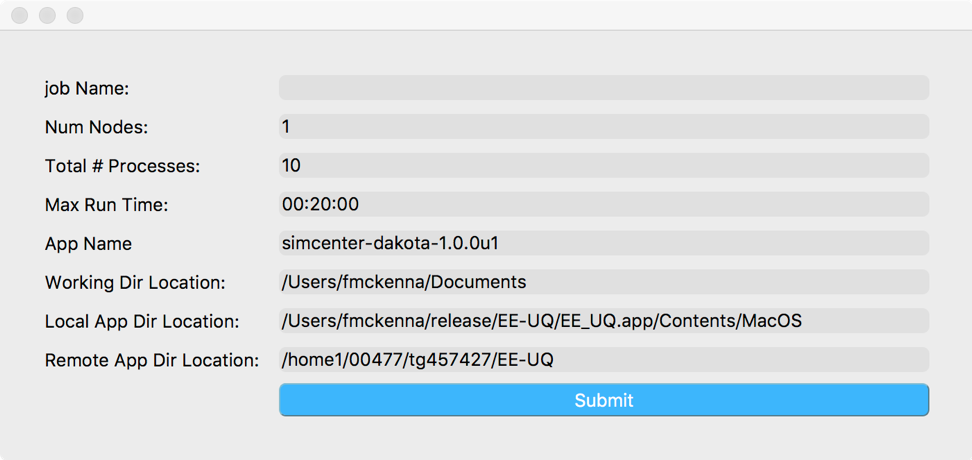
\includegraphics[width=0.8\textwidth]
    {figs/Figure16.png} }
  \caption{Remote button}
  \label{fig:figure16}
\end{figure}

A similar bit longer input panel is brought up:
\begin{itemize}
\item JobName: The name the user can use to identify the job in Get from DesignSafe.
\item NumNodes: The number of compute nodes to use on Stampede2. Using the default App Name the job will run on Stampede2’s KNL Landing (KNL) 
compute nodes. Each node has 68 cores. The actual number of cores the application will use on each of these nodes depends on the total number of 
processes specified. As per the TACC webpage, for MPI tasks it’s best not to specify more than 64-68 processes to run. Depending on the numerical 
computations and amount of memory each uses, so as to avoid page faulting, for large simulations you may wish to use more nodes and less processes.
\item Total Number of Processes: Total number of MPI parallel processes the UQ engine is going to use.
\item Max Wall Time:  HOURS:MIN:SEC be conservative. Your job is killed after the time limit. On Stampede2 you have a max wall time of 24 hours.
\item App Name:   Name of Agave app to run. DO not touch unless you know what you are doing.
\item Working Dir Location: specifies where the $EE_UQ$ application can create a “temporary” directory called tmp. SimCenter that the application 
creates when the submit button is pressed. The application creates this directory, copies files to it that the application needs as a result of your 
input (e.g. if you are using OpenSees input script, it will to the tmp. SimCenter directory copy that script, ALL FILES IN THAT DIRECTORY AND ALL FILES 
IN SUBDIRECTORIES OF THAT DIRECTORY. (SO, DON’T PLACE THE SCRIPT IN HOME, DOWNLOADS, DOCUMENTS, …). That directory is removed when jib has been successfully submitted.
\item Local App Dir Location: SHOULD NOT BE TOUCHED unless you are introducing your own applications or want to build and modify the applications 
provided with the tool. It is this directory the application tool looks to find the applications it needs.
\item Remote App Dir Location: Remote directory on Stampede2 where applications needed by workflow reside. DO not touch unless you know what you are doing.

\end{itemize}


\subsection{GET from DesignSafe}
	Click this button to obtain from DesignSafe your list of jobs and select from that list a job to update status of, download or delete.

\subsection{Exit}
Click this button to exit the application. 
